% ::setlocal makeprg=cd\ presentazione\ &&\ pdflatex\ -interaction=batchmode\ main.tex\ &&\ okular\ main.pdf\ &

\section{Introduzione}


\begin{frame}{Introduzione}
    \begin{itemize}
        \item Cos'è la relatività generale e perché esiste
        \item Cos'è la metrica di \Sh
        \item Studio delle geodetiche come strumento per capire la metrica
        \item Soluzioni numeriche alle equazioni del moto di una particella
            massiva
    \end{itemize}
\end{frame}


\begin{frame}{Il moto di una particella libera}

    Possiamo descrivere il moto di una particella libera tramite il principio
    variazionale \\

    \begin{block}{Principio di Minima Azione}
        {Una particella libera che si muove da $A$ a $B$ segue il percorso che
        minimizza la distanza tra i due punti.}
    \end{block}

    ~

    Il problema si può quindi ricondurre a come si misura \textit{correttamente}
    una \textbf{distanza}?

\end{frame}


\begin{frame}{Misurare le Distanze}
\begin{minipage}{0.49\textwidth}
    \center{Meccanica Newtoniana}
    \begin{equation*}
        \dd s^2 = \dd x^2 + \dd y^2 + \dd z^2
    \end{equation*}
    \begin{figure}
        \centering
        \begin{tikzpicture}[scale=0.8]
            % Axes
            \draw[->] (0, 0) -- (5, 0) node[below right] {$x$};
            \draw[->] (0, 0) -- (0, 4) node[above left] {$y$};
            
            % Points
            \coordinate (A) at (1, 1);
            \coordinate (B) at (4, 3);
            \filldraw[blue] (A) circle (2pt) node[below left] {A};
            \filldraw[red] (B) circle (2pt) node[above right] {B};
            
            % Lines
            \draw[] (A) -- (B) node[midway, above, sloped] {$\Delta s$};
            \draw[dashed] (A) -- (4, 1) -- (B);
            
            % Labels
            \node[below] at (2.5, 1) {$\Delta x$};
            \node[right] at (4, 2) {$\Delta y$};
            
        \end{tikzpicture}
        \caption{Rappresentazione 2D ($x$, $y$) di $\Delta s^2$.}
    \end{figure}
\end{minipage}
\pause
\begin{minipage}{0.49\textwidth}
    \center{Relatività Ristretta}
    \begin{equation*}
        \dd s^2 = - c^2 \dd t^2 + \dd x^2 + \dd y^2 + \dd z^2
    \end{equation*}
    \begin{figure}
        \centering
        \begin{tikzpicture}[scale=0.8]
            % Axes
            \draw[->] (0, 0) -- (5, 0) node[below right] {$x$};
            \draw[->] (0, 0) -- (0, 4) node[above left] {$ct$};
            
            % Points
            \coordinate (A) at (1, 1);
            \coordinate (B) at (4, 3);
            \filldraw[blue] (A) circle (2pt) node[below left] {A};
            \filldraw[red] (B) circle (2pt) node[above right] {B};
            
            % Lines
            \draw[] (A) -- (B) node[midway, above, sloped] {$\Delta s$};
            \draw[dashed] (A) -- (4, 1) -- (B);
            
            % Labels
            \node[below] at (2.5, 1) {$\Delta x$};
            \node[right] at (4, 2) {$c \Delta t$};
            
        \end{tikzpicture}
        \caption{Rappresentazione 2D ($x$, $ct$) di $\Delta s^2$.}
    \end{figure}
\end{minipage}
\end{frame}


\begin{frame}{Riformulazione della Meccanica}

    \`E utile definire la metrica

    \begin{equation*}
        \eta_{\nu \mu} = 
        \begin{array}{cc}
            \begin{pNiceMatrix}[first-row,first-col][columns-width = auto]
                  & t & x & y & z \\
                t~~ & -1 & 0 & 0 & 0 \\  
                x~~ & 0 & 1 & 0 & 0 \\ 
                y~~ & 0 & 0 & 1 & 0 \\
                z~~ & 0 & 0 & 0 & 1 \\
            \end{pNiceMatrix} &
        \end{array}
        \quad \implies \quad
        \mathrm{d}s^2 = \eta_{\nu \mu} \mathrm{d}x^\nu \mathrm{d}x^\mu
    \end{equation*}

    \vspace{1cm}

    $\dd s^2$ si chiama \textbf{elemento di linea}, ha le seguenti proprietà:

    \begin{itemize}
        \item è uguale per tutti i sistemi di riferimento inerziali
        \item determina la geometria dello spaziotempo
    \end{itemize}

\end{frame}


\begin{frame}{Il Problema della Forza di Gravità}

    La forza di gravità tra due masse $m_1$ e $m_2$, posizionate in $r_1(t)$ e
    $r_2(t)$, \textbf{non è compatibile con la relatività ristretta}. Infatti

    \vspace{1cm}

    \begin{equation*}
        F_{12} = G \frac{m_1 m_2}{|r_1(t) - r_2(t)|^2}
    \end{equation*}

    \vspace{1cm}

    \begin{itemize}
        \item Nella teoria di Newton dovrebbe essere istantanea
        \item $\abs{r_1(t) - r_2(t)}$ dipende dal sistema di riferimento
    \end{itemize}

\end{frame}


\begin{frame}{Una Nuova Teoria}

    \begin{block}{Relatività Generale}
        {La massa di un oggetto non da origine alla forza di gravità, ma curva
        lo \textit{spaziotempo} stesso.}
    \end{block}

    L'elemento di linea $\dd s^2$ si dovrà calcolare in modo diverso.

    \begin{figure}
        \centering
        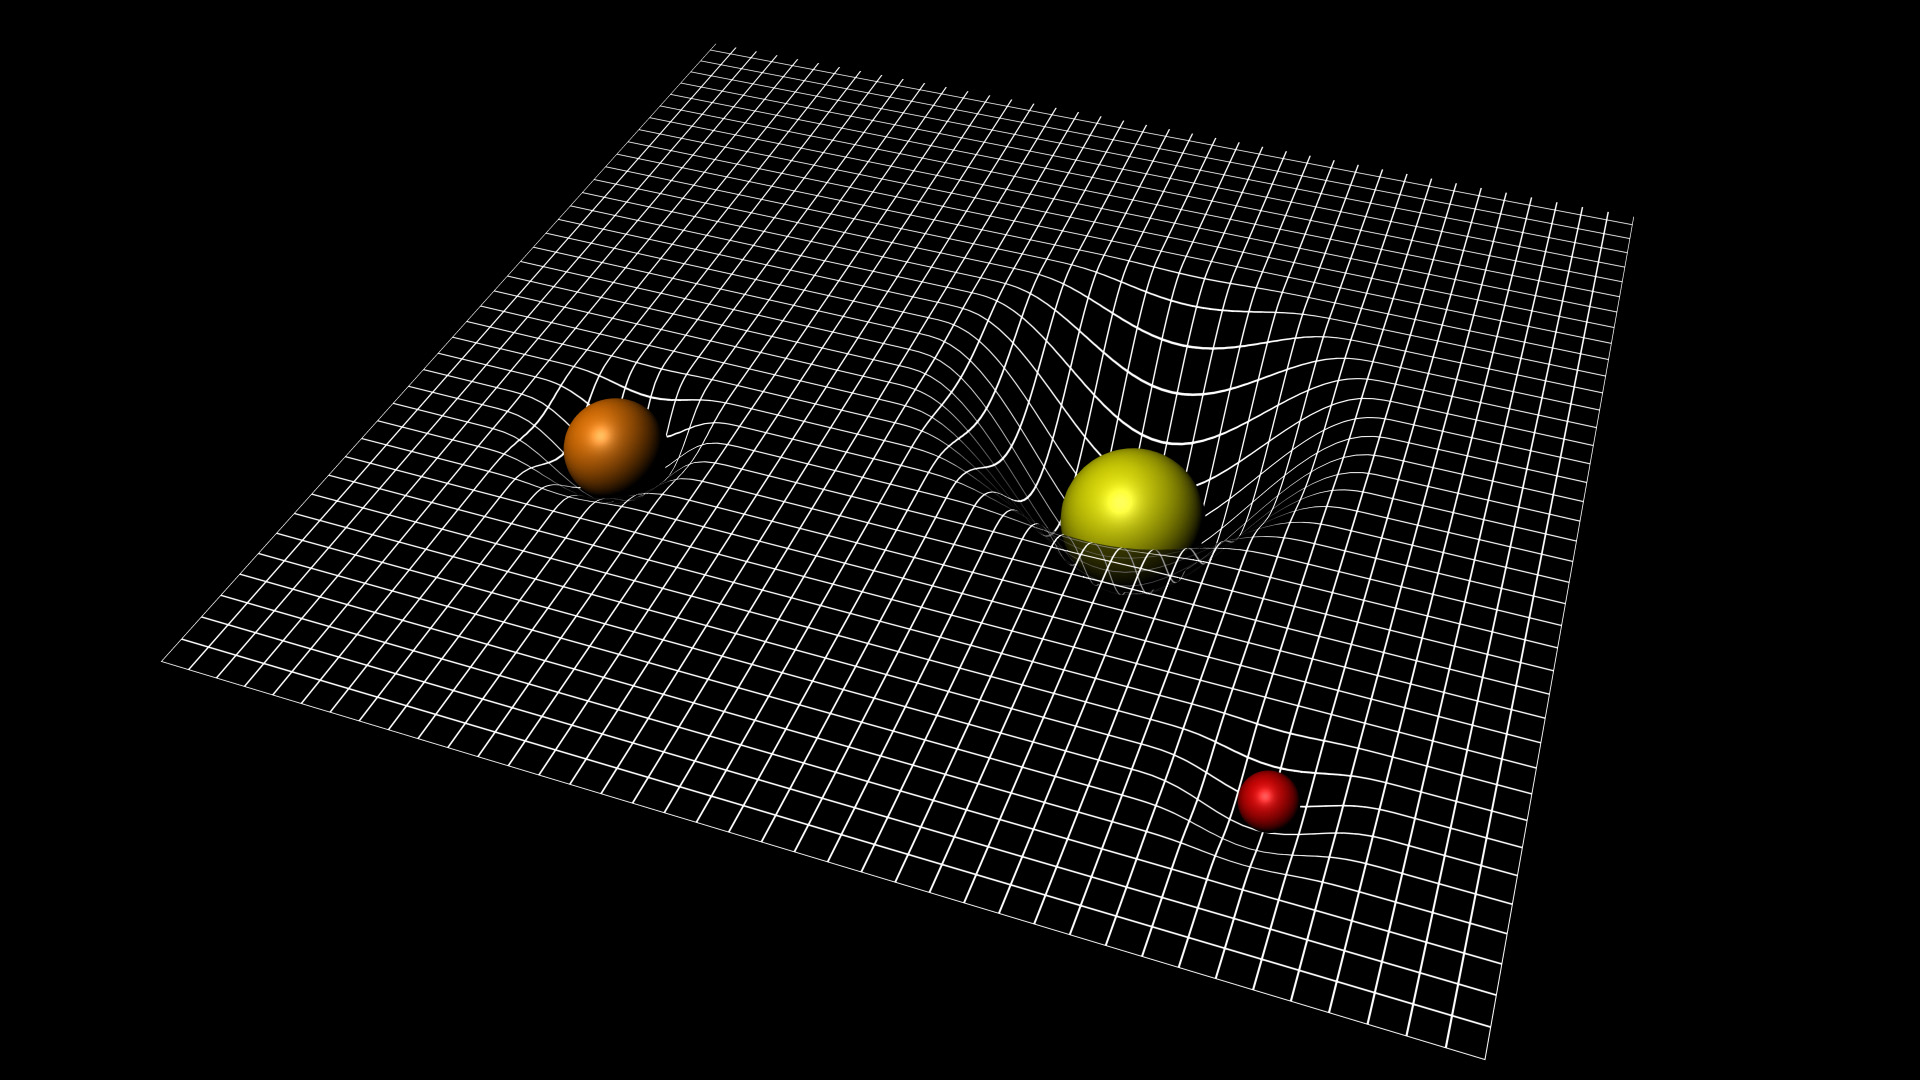
\includegraphics[width=0.7\textwidth]{Figures/spacetime_curvature.jpg}
        \caption{\textit{https://www.esa.int}}%/ESA\_Multimedia/Images/2015/09/Spacetime\_curvature}}
    \end{figure}

\end{frame}


\begin{frame}{Il Moto nello Spazio Curvo}
    La distanza più breve tra due punti in uno spazio curvo non è più una retta
    \begin{figure}
        \centering
        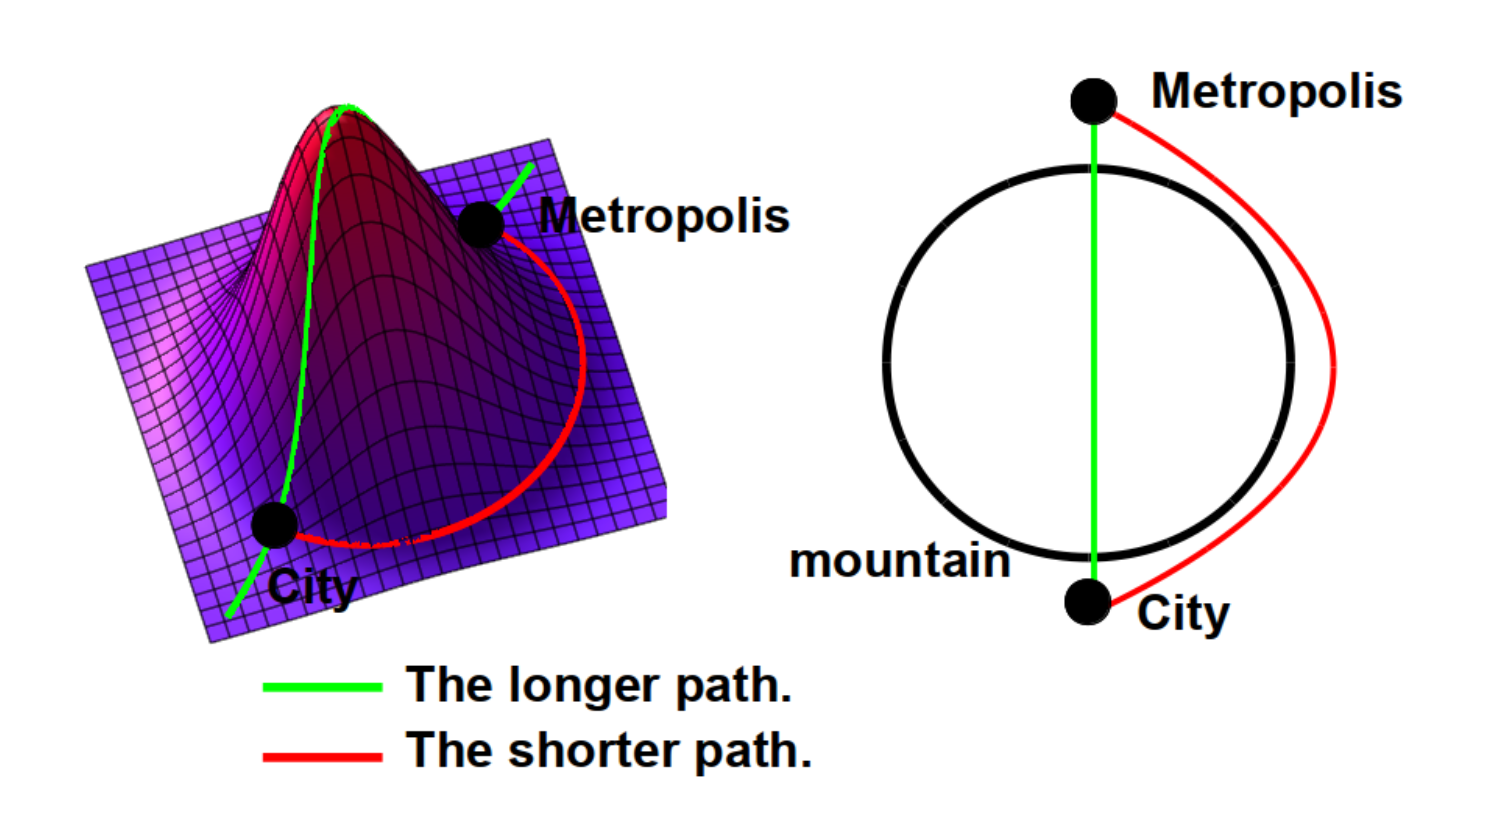
\includegraphics[width=0.7\textwidth]{Figures/moutain_curved_space.png}
        \caption{\textit{https://www.thephysicsmill.com}}%/2015/08/15/general-relativity-is-the-curvature-of-spacetime/}}
    \end{figure}

\end{frame}
